\documentclass[10pt,fleqn]{article}
\newcommand{\name}[1]{\def\psettitlename{#1}}
\newcommand{\course}[1]{\def\psettitlecourse{#1}}
\newcommand{\rsection}[1]{\def\psettitlersection{#1}}
\newcommand{\psetnum}[1]{\def\psettitlepsetnum{#1}}
% \usepackage[journal=rsc]{chemstyle}
% \usepackage{mhchem}
\usepackage{amsmath}
\usepackage{amssymb}
\usepackage{amsfonts}
\usepackage{esint}
\usepackage{bbm}
\usepackage{amscd}
\usepackage{picinpar}
\usepackage[pdftex]{graphicx}
\usepackage{indentfirst}
\usepackage{wrapfig}
\usepackage{units}
\usepackage{textcomp}
\usepackage[utf8x]{inputenc}
\usepackage{feyn}
\usepackage{feynmp}
\DeclareGraphicsRule{*}{mps}{*}{}
\newcommand{\ud}{\mathrm{d}}
\newcommand{\ue}{\mathrm{e}}
\newcommand{\ui}{\mathrm{i}}
\newcommand{\res}{\mathrm{Res}}
\newcommand{\Tr}{\mathrm{Tr}}
\newcommand{\dsum}{\displaystyle\sum}
\newcommand{\dprod}{\displaystyle\prod}
\newcommand{\dlim}{\displaystyle\lim}
\newcommand{\dint}{\displaystyle\int}
\newcommand{\fsno}[1]{{\!\not\!{#1}}}
\newcommand{\eqar}[1]
{
  \begin{align*}
    #1
  \end{align*}
}
\newcommand{\texp}[2]{\ensuremath{{#1}\times10^{#2}}}
\newcommand{\dexp}[2]{\ensuremath{{#1}\cdot10^{#2}}}
\newcommand{\eval}[2]{{\left.{#1}\right|_{#2}}}
\newcommand{\paren}[1]{{\left({#1}\right)}}
\newcommand{\lparen}[1]{{\left({#1}\right.}}
\newcommand{\rparen}[1]{{\left.{#1}\right)}}
\newcommand{\abs}[1]{{\left|{#1}\right|}}
\newcommand{\sqr}[1]{{\left[{#1}\right]}}
\newcommand{\crly}[1]{{\left\{{#1}\right\}}}
\newcommand{\angl}[1]{{\left\langle{#1}\right\rangle}}
\newcommand{\tpdiff}[4][{}]{{\paren{\frac{\partial^{#1} {#2}}{\partial {#3}{}^{#1}}}_{#4}}}
\newcommand{\tpsdiff}[4][{}]{{\paren{\frac{\partial^{#1}}{\partial {#3}{}^{#1}}{#2}}_{#4}}}
\newcommand{\pdiff}[3][{}]{{\frac{\partial^{#1} {#2}}{\partial {#3}{}^{#1}}}}
\newcommand{\diff}[3][{}]{{\frac{\ud^{#1} {#2}}{\ud {#3}{}^{#1}}}}
\newcommand{\psdiff}[3][{}]{{\frac{\partial^{#1}}{\partial {#3}{}^{#1}} {#2}}}
\newcommand{\sdiff}[3][{}]{{\frac{\ud^{#1}}{\ud {#3}{}^{#1}} {#2}}}
\newcommand{\tpddiff}[4][{}]{{\left(\dfrac{\partial^{#1} {#2}}{\partial {#3}{}^{#1}}\right)_{#4}}}
\newcommand{\tpsddiff}[4][{}]{{\paren{\dfrac{\partial^{#1}}{\partial {#3}{}^{#1}}{#2}}_{#4}}}
\newcommand{\pddiff}[3][{}]{{\dfrac{\partial^{#1} {#2}}{\partial {#3}{}^{#1}}}}
\newcommand{\ddiff}[3][{}]{{\dfrac{\ud^{#1} {#2}}{\ud {#3}{}^{#1}}}}
\newcommand{\psddiff}[3][{}]{{\frac{\partial^{#1}}{\partial{}^{#1} {#3}} {#2}}}
\newcommand{\sddiff}[3][{}]{{\frac{\ud^{#1}}{\ud {#3}{}^{#1}} {#2}}}
\usepackage{fancyhdr}
\usepackage{multirow}
\usepackage{fontenc}
% \usepackage{tipa}
\usepackage{ulem}
\usepackage{color}
\usepackage{cancel}
\newcommand{\hcancel}[2][black]{\setbox0=\hbox{#2}%
  \rlap{\raisebox{.45\ht0}{\textcolor{#1}{\rule{\wd0}{1pt}}}}#2}
\pagestyle{fancy}
\setlength{\headheight}{67pt}
\fancyhead{}
\fancyfoot{}
\fancyfoot[C]{\thepage}
\fancyhead[R]
{
  \psettitlename \\
  \psettitlecourse{} Problem Set \psettitlepsetnum \\
  \ifx\psettitlersection\empty
  \else
  Recitation Section \psettitlersection
  \fi
}
\renewcommand{\footruleskip}{0pt}
\renewcommand{\headrulewidth}{0.4pt}
\renewcommand{\footrulewidth}{0pt}
\addtolength{\hoffset}{-1.3cm}
\addtolength{\voffset}{-2cm}
\addtolength{\textwidth}{3cm}
\addtolength{\textheight}{2.5cm}
\renewcommand{\footskip}{10pt}
\setlength{\headwidth}{\textwidth}
\setlength{\headsep}{20pt}
\setlength{\marginparwidth}{0pt}
\parindent=0pt
\psetnum{1}
\course{Physics 251b}
\rsection{1}
\name{Yichao Yu}
\renewcommand{\thesection}{\arabic{section}.}
\renewcommand{\thesubsection}{(\alph{subsection})}
\renewcommand{\thesubsubsection}{\roman{subsubsection}.}

\begin{document}
\section{}
\subsection{}
Represent the operation using $4\times4$ matrices that shows the mapping between
the nodes.
\eqar{
  T_1=&\begin{pmatrix}
    1&&&\\
    &1&&\\
    &&1&\\
    &&&1
  \end{pmatrix}&T_2=&\begin{pmatrix}
    1&&&\\
    &&1&\\
    &&&1\\
    &1&&
  \end{pmatrix}&T_3=&\begin{pmatrix}
    1&&&\\
    &&&1\\
    &1&&\\
    &&1&
  \end{pmatrix}\\
  T_4=&\begin{pmatrix}
    &1&&\\
    1&&&\\
    &&&1\\
    &&1&
  \end{pmatrix}&T_5=&\begin{pmatrix}
    &1&&\\
    &&1&\\
    1&&&\\
    &&&1
  \end{pmatrix}&T_6=&\begin{pmatrix}
    &1&&\\
    &&&1\\
    &&1&\\
    1&&&
  \end{pmatrix}\\
  T_7=&\begin{pmatrix}
    &&1&\\
    1&&&\\
    &1&&\\
    &&&1
  \end{pmatrix}&T_8=&\begin{pmatrix}
    &&1&\\
    &1&&\\
    &&&1\\
    1&&&
  \end{pmatrix}&T_9=&\begin{pmatrix}
    &&1&\\
    &&&1\\
    1&&&\\
    &1&&
  \end{pmatrix}\\
  T_{10}=&\begin{pmatrix}
    &&&1\\
    1&&&\\
    &&1&\\
    &1&&
  \end{pmatrix}&T_{11}=&\begin{pmatrix}
    &&&1\\
    &&1&\\
    &1&&\\
    1&&&
  \end{pmatrix}&T_{12}=&\begin{pmatrix}
    &&&1\\
    &1&&\\
    1&&&\\
    &&1&
  \end{pmatrix}
}
\subsection{}
\eqar{
  g_{123}=&\begin{pmatrix}
    &&1&\\
    1&&&\\
    &1&&\\
    &&&1
  \end{pmatrix}\\g_{234}=&\begin{pmatrix}
    1&&&\\
    &&&1\\
    &1&&\\
    &&1&
  \end{pmatrix}\\
  g_{234}g_{123}=&\begin{pmatrix}
    &1&&\\
    1&&&\\
    &&&1\\
    &&1&
  \end{pmatrix}=T_4
}
($180^\circ$ rotation around the the axis connecting the middle of 1-2 and 3-4)
\eqar{
  g_{123}g_{234}=&\begin{pmatrix}
    &&1&\\
    &&&1\\
    1&&&\\
    &1&&
  \end{pmatrix}=T_9\neq T_4
}
\subsection{}
See (a)
\subsection{}
\eqar{
  H=\begin{pmatrix}
    \varepsilon_0&-t&-t&-t\\
    -t&\varepsilon_0&-t&-t\\
    -t&-t&\varepsilon_0&-t\\
    -t&-t&-t&\varepsilon_0
  \end{pmatrix}
}
Eigenvalues are $\varepsilon_0-3t$ for eigenvector $\paren{\dfrac12,\dfrac12,\dfrac12,\dfrac12}$ and $\varepsilon_0+t$ for eigenvectors, $\paren{\dfrac12,\dfrac12,-\dfrac12,-\dfrac12}$, $\paren{\dfrac12,-\dfrac12,\dfrac12,-\dfrac12}$, $\paren{\dfrac12,-\dfrac12,-\dfrac12,\dfrac12}$.
\section{}
\subsection{}
\eqar{
  H=\begin{pmatrix}
    \varepsilon_0&-t&&&&-t&&-t\\
    -t&\varepsilon_0&-t&&-t&&&\\
    &-t&\varepsilon_0&-t&&&&-t\\
    &&-t&\varepsilon_0&-t&&-t&\\
    &-t&&-t&\varepsilon_0&-t&&\\
    -t&&&&-t&\varepsilon_0&-t&\\
    &&&-t&&-t&\varepsilon_0&-t\\
    -t&&-t&&&&-t&\varepsilon_0
  \end{pmatrix}
}
Eigenvalues and eigenvectors are,
$\lambda_1=\varepsilon_0-3t$,
\eqar{
  v_1=&\frac{1}{2\sqrt 2}\begin{pmatrix}1&1&1&1&1&1&1&1\end{pmatrix}
}
$\lambda_2=\varepsilon_0+3t$,
\eqar{
  v_2=&\frac{1}{2\sqrt 2}\begin{pmatrix}1&-1&1&-1&1&-1&1&-1\end{pmatrix}
}
$\lambda_{3,4,5}=\varepsilon_0-t$ (3-fold degenerate)
\eqar{
  v_{3}=&\frac{1}{2}\begin{pmatrix}1&0&0&-1&-1&0&0&1\end{pmatrix}\\
  v_{4}=&\frac{1}{2}\begin{pmatrix}-1&-1&0&1&0&0&1&0\end{pmatrix}\\
  v_{5}=&\frac{1}{2}\begin{pmatrix}1&0&-1&-1&0&1&0&0\end{pmatrix}
}
and $\varepsilon_0+t$ (3-fold degenerate)
\eqar{
  v_{6}=&\frac{1}{2}\begin{pmatrix}-1&0&0&-1&1&0&0&1\end{pmatrix}\\
  v_{7}=&\frac{1}{2}\begin{pmatrix}-1&1&0&-1&0&0&1&0\end{pmatrix}\\
  v_{8}=&\frac{1}{2}\begin{pmatrix}-1&0&1&-1&0&1&0&0\end{pmatrix}
}
\subsection{}
$\varepsilon_0-3t$ corresponds to the $A_1$ representation.\\
$\varepsilon_0+3t$ corresponds to the $A_2$ representation.\\
$\varepsilon_0-t$ corresponds to the $T_1$ representation.\\
$\varepsilon_0+t$ corresponds to the $T_2$ representation.
\subsection{}
From the form of the Hamiltonian,
\eqar{
  \lambda_j=&\varepsilon_0+\lambda_j(0,t,t')\\
  \lambda_j(0,kt,kt')=&k\lambda_j(0,t,t')\\
  \lambda_j(0,t,t')=&t\lambda_j(0,1,t'/t)\\
  =&f_j(t'/t)
}
Plot,\\
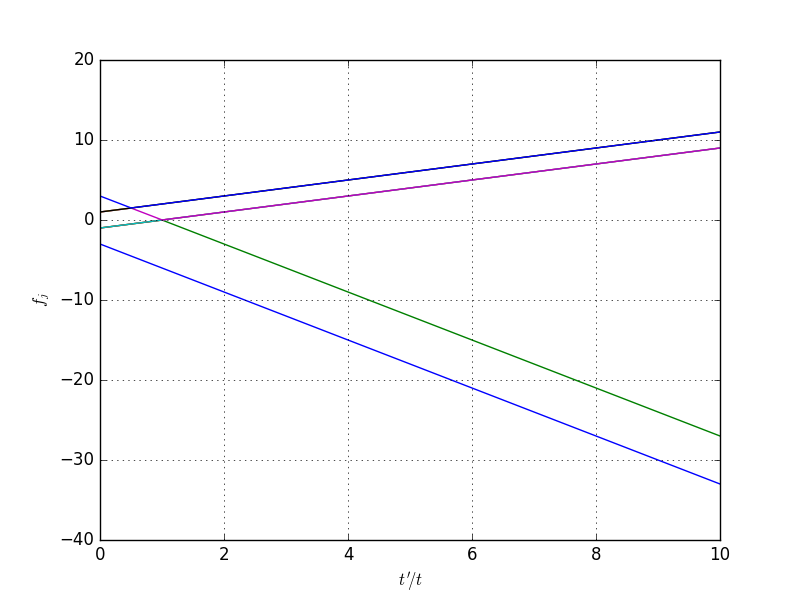
\includegraphics[width=8cm]{p2c.png}\\
There is accidental degeneracy for certain parameters.
\section{}
The constrains is that the angular momentum cannot perfectly point in a certain
direction and there will always be some fluctuations. This uncertain comes from,
\eqar{
  \angl{\Delta L_x, \Delta L_y}\geqslant&\frac1{2\ui}\angl{\sqr{L_x, L_y}}\\
  =&\frac{\hbar}{2}\angl{L_z}\\
  =&\frac{\hbar^2m}{2}
}
Which can only be $0$ when $m=0$.
\section{}
\subsection{}
Define $g(\phi, \phi_0)\equiv\ue^{-\ui L_z\phi_0/\hbar}f(\phi)$
\eqar{
  \pdiff{g}{\phi_0}=&-\frac{\ui L_z}{\hbar}\ue^{-\ui L_z\phi_0/\hbar}f(\phi)\\
  =&-\pdiff{}{\phi}\ue^{-\ui L_z\phi_0/\hbar}f(\phi)\\
  =&-\pdiff{g}{\phi}\\
  \ud g=&\pdiff{g}{\phi_0}\ud\phi_0+\pdiff{g}{\phi}\ud\phi\\
  =&\pdiff{g}{\phi}\paren{\ud\phi-\ud\phi_0}
}
Therefore $g=g(\phi-\phi_0)$ (since it has $0$ gradient in this direction).
Since $g(\phi) = f(\phi)$ (when $\phi_0 = 0$), $g(\phi, \phi_0) = f(\phi - \phi_0)$ for all $\phi_0$.
\subsection{}
Define $\sigma_n\equiv\sigma\cdot\hat n$
\eqar{
  \paren{\sigma\cdot\hat n}^2=&n_x^2 + n_y^2 + n_z^2\\
  =&1
}
(using the fact that $\sigma_i$'s anti-commutes with each other)
\eqar{
  \ue^{-\ui\sigma_n\varphi/2}=&\sum_{j=0}^\infty\frac{\paren{-\ui\sigma_n\varphi/2}^j}{j!}\\
  =&\sum_{j=0}^\infty\frac{\paren{-\ui\sigma_n\varphi/2}^{2j}}{(2j)!}+\sum_{j=0}^\infty\frac{\paren{-\ui\sigma_n\varphi/2}^{2j+1}}{(2j+1)!}\\
  =&\sum_{j=0}^\infty\frac{\paren{-1}^{j}\paren{\varphi/2}^{2j}}{(2j)!}-\ui\sigma_n\sum_{j=0}^\infty\frac{\paren{-1}^{j}\paren{\varphi/2}^{2j+1}}{(2j+1)!}\\
  =&\cos\frac{\varphi}{2}-\ui\sigma_n\sin\frac{\varphi}{2}
}
\subsection{}
\eqar{
  T_{x180}=&\ue^{-\ui\sigma_x\pi/2}\\
  =&\cos\frac{\pi}{2}-\ui\sigma_x\sin\frac{\pi}{2}\\
  =&-\ui\sigma_x
}
which switches up and down spin with a phase factor. Spining around y-axis gives the same spin flip with a different phase factor.
\subsection{}
\eqar{
  T_{x90}=&\ue^{-\ui\sigma_x\pi/4}\\
  =&\cos\frac{\pi}{4}-\ui\sigma_x\sin\frac{\pi}{4}\\
  =&\frac{1}{\sqrt{2}}\paren{1-\ui\sigma_x}
  \intertext{The effect on $\chi^+$,}
  T_{x90}\chi^+=&\frac{1}{\sqrt{2}}\paren{1-\ui\sigma_x}\chi^+\\
  =&\frac{1}{\sqrt{2}}\paren{\chi^+-\ui\chi^-}
}
\subsection{}
\eqar{
  T_{z180}=&\ue^{-\ui\sigma_z\pi}\\
  =&\cos\pi-\ui\sigma_z\sin\pi\\
  =&-1
}
The global phase has no observable effect on this system.
It could have non-trivial effect if it is possible to interfere this system
with another one.
\section{}
\subsection{}
For $n=0$, $\sqr{A, B^0}=0$ is true.
When the equation is true for $n-1$ we have,
\eqar{
  \sqr{A, B^n}=&\sqr{A, B^{n-1}B}\\
  =&\sqr{A, B^{n-1}}B+B^{n-1}\sqr{A, B}\\
  =&\paren{n-1}B^{n-2}\sqr{A, B}B+B^{n-1}\sqr{A, B}\\
  =&\paren{n-1}B^{n-1}\sqr{A, B}+B^{n-1}\sqr{A, B}\\
  =&nB^{n-1}\sqr{A, B}
}
So the equation is true for $n$ as well. Therefore, the equation is true for all non-negative finite $n$.\\

Assume $f(x)\equiv\dsum_{n=0}^\infty a_nx^n$
\eqar{
  \sqr{p_x, f(x)}=&\sqr{p_x, \dsum_{n=0}^\infty a_nx^n}\\
  =&\dsum_{n=0}^\infty \sqr{p_x, a_nx^n}\\
  =&-\ui\hbar\dsum_{n=0}^\infty a_nnx^{n-1}\\
  =&-\ui\hbar\dsum_{n=0}^\infty a_n\pdiff{x^n}{x}\\
  =&-\ui\hbar\pdiff{}{x}\dsum_{n=0}^\infty a_nx^n\\
  =&-\ui\hbar\pdiff{f(x)}{x}
}
\subsection{}
\eqar{
  \diff{}{t}\vec L_{op}=&\frac{\ui}{\hbar}\sqr{H, \vec L}\\
  =&\frac{\ui}{\hbar}\sqr{\frac{p^2}{2m}+V, \vec x\times\vec p}\\
  =&\frac{\ui}{\hbar}\sqr{\frac{p^2}{2m}, \vec x}\times\vec p+\frac{\ui}{\hbar}\vec x\times\sqr{V, \vec p}\\
  =&\frac{-\ui}{2m\hbar}2\ui\hbar\vec p\times\vec p+\frac{\ui}{\hbar}\vec x\times\ui\hbar\nabla V\\
  =&-\vec x\times\nabla V\\
  =&\vec N_{op}
}
\subsection{}
If $V$ is spherically symmetric, $\nabla V\parallel\vec x$ so $\vec N_{op}=-\vec x\times\nabla V=0$ (since everything commutes...)
\end{document}
